\begin{artengenv}
	{Tadeusz Sierotowicz}
	{Where are Sunspots? The Practical Method of Galileo as an example of Mental Model}
	{Where are Sunspots? The Practical Method of Galileo\ldots}
	{Where are Sunspots? The Practical Method of Galileo as an example of Mental Model}
	{Copernicus Center for Interdisciplinary Studies,\\
		Istituto di Scienze Religiose di Bolzano e IISS Gandhi di Merano}
	{After the publication of \textit{Sidereus Nuncius} Galileo, in the controversy with Ch.
		Scheiner, developed several arguments on behalf of the hypothesis that sunspots are contiguous to the surface of the
		Sun, and presented them in his \textit{Istoria e dimostrazioni intorno alle macchie solari e loro accidenti}
		(Roma 1613). One of them, named by Galileo a Practical Method, advocates very clearly the correctness of the
		hypothesis. In the paper the method in question is briefly described. It is argued that the Practical Method is not a
		thought experiment, but rather a mental model proposed precisely in order to solve the problem of sunspots’ location. }
	{sunspots, Galileo’s practical method, mental models, early modern science.}
















\section{Introduction}

\lettrine[loversize=0.13,lines=2,lraise=-0.03,nindent=0em,findent=0.2pt]%
{A}{}fter Galileo discovered many celestial novelties through his telescope, as described in the widely read
\textit{Sidereus Nuncius}, his \textit{vis polemica} found a space in the sunspot dispute with the Jesuit priest
Christopher Scheiner \label{ref:RNDsvmOJdj55M}(Camerota, 2004, pp.238–259; Fantoli, 2003, chap.2.6; Heilbron, 2010,
pp.183–192; Galilei and Scheiner, 2010; Shea, 1970; Sierotowicz, 2013)\footnote{ Bibliographical note: the
\textit{opera} of Galileo Galilei discussed in the paper can be easily found on the Web: \textit{Istoria e
dimostrazioni…}, \label{ref:RNDAJ1gfHi67B}(Galilei, 1613) see, e.g., copy of the National Library of Florence: BNCF -
II 461, the Nencini collection: brunelleschi.imss.fi.it/bibliotecagalileo; [\textcolor{black}{Accessed 23 Dec. 2010]}.
In the national edition of the works of Galilei, \textit{Istoria e dimostrazioni…} can be found in the fifth volume:
\label{ref:RNDZuSZALA3Op}(Favaro, 1895, pp.25–239). Favaro’s edition is cited here with the abbreviation OG, followed
by the number of the volume, the page number, and the verse number. For the English translation, see
\label{ref:RNDD928OnAcs5}(Galilei, 2010). Figures: For all details, see \label{ref:RNDJx6FkG6s8J}(Sierotowicz, 2013).
}. In this article, I pay special attention to a few pages from \textit{Istoria e dimostrazioni intorno alle macchie
solari e loro accidenti} \label{ref:RNDsCgxW6zxj5}(Galilei, 1613), which has been largely neglected by scholars. In the
work, the Pisano\footnote{ Galileo is often referred to as the Pisano, after the city of his birth.} presented what he
himself called the most powerful reason in favour of his thesis about the location of sunspots. This is an original
method, called the Practical Method \label{ref:RNDHr9m3pOWbB}(see OG V, 121.5; Galilei, 2010, p.112), through which
Galileo tried to prove his hypothesis by combining in a paradigmatic way sensible experiences (observations) and
necessary demonstrations (a geometrical model).

Galileo Galilei, in opposition to Christopher Scheiner, considered sunspots a phenomenon that exist on the surface of
the Sun and, as a consequence, participate in the rotation of the solar globe. However, according to Scheiner, sunspots
are just shadows of the passage of planets distant from the Sun through the solar disk. All these planets have to move
with an angular velocity that is equal to the angular velocity of the rotation of the Sun.

To decide which of these two theories is right, Galileo proposed several arguments. One of them, a sort of cinematic and
geometric reasoning, was based on the variation of the relative distance between the two spots moving along the same
parallel from the edge of the solar disk towards its centre. The Pisano noted that the observed distance between such
two sunspots changes in a particular way because of the projection on the observation plane of the segment between the
spots according to the angle that the segment forms with the plane of observation. Galileo developed a geometrical
model of this situation in his work on sunspots mentioned above (Fig 1). 

The apparent distance between two sunspots is normally smaller than the actual distance between them. However, on one
occasion, namely, when the segment between two spots is parallel to the observation plane, the length of the segment
and the length of its orthogonal projection onto the observation plane will be the same. This happens when the straight
line joining the observer’s eye with the centre of the Sun is aligned with the centre of the segment that joins the
spots (Fig. 5). Of course, this situation is rather exceptional, but Galileo was lucky enough to observe it for two
sunspots on 01 July 1613 and 05 July 1613, respectively (Fig. 2 and 3). Extraordinary, masterly executed drawings
representing these observations were printed in \textit{Istoria e dimostrazioni…. }In fact, on July 5, 1613, spots A
and B appeared to be symmetrically located with respect to the centre of the solar disk. This particular observation
allowed Galileo to develop and apply the Practical Method. 

\section{The Practical Method}

First, Galileo noted that «because the distance between the Sun and us is very great in proportion to the diameter of
its body» \label{ref:RNDRTm53mTJKP}(OG V, 121; Galilei, 2010, p.112) some preliminary premises, also of a physical
nature, for his model can be made: 

(1) The rays that reach the eye of the terrestrial observer can be considered as parallel lines (see the rays ZDG, OLI,
and QP in Fig. 1);

(2) Sunspots are located on the same latitude and pass through the centre of the solar disk or very close to it; and

(3) This situation occurs in the case of two spots, A and B (see Fig. 2 and 3).

Starting with these suppositions, Galileo constructed the geometric model of sunspot observations. The plane of the
drawing (Fig. 1) corresponds to the plane passing through the observer, the centre of the Sun, and the parallel
(practically the equator) on which the sunspots A and B are located. The GDZ line, coming out from the centre of the
Sun G, goes towards the terrestrial observer to whom the spots appear projected on the plane perpendicular to the plane
just mentioned and passing through the centre of the Sun (the observation plane). Let CDE be the semicircle
representing the surface of the Sun, or the parallel on which the A and B spots move, and let the points on the CGE
segment correspond to the observed positions of sunspots in an orthogonal projection on the observation plane. The
points L and H are the sunspots A and B, respectively, observed on 01 July 1613 (Fig. 2). The actual distance between
these spots is equal to the HL chord, but because of the projection effects, these spots are observed as points F and
I, and their observed distance is equal to the length of the FI segment. It is easy to see that in a situation where
the HL segment is symmetrical with respect to the GDZ line, the observed distance should be equal to the length of the
HL segment because the HL, FI, and CGE segments are parallel. This situation actually occurred on 5 July 1613 (see Fig.
3 and 5).

Naturally, the construction described above corresponds to the hypothesis that sunspots are supposed to be located on
the surface of the Sun, or very near to it. What if the spots are but the shadows of a distant planet (Scheiner’s
hypothesis)? Let us now imagine that the phenomenon of the spots is caused by a transition through the solar disk of
objects distant from the surface of the Sun that are about 1/20th of the diameter of the solar disk. The objects in
question therefore move on the MNO semicircle (Fig. 1). In this case, sunspots should be collocated in points N and O,
and their real distance should correspond to the segment NO. It is easy to find out using a compass that the segment NO
is shorter than the HL one. Nevertheless, even in this case, the observed distance corresponds to the FI segment
because the geometric construction represents the way in which the mind and the eye of the terrestrial observer builds
images of the spots. How to decide which of the two situations, clearly different, reflects the real situation? To put
it briefly: where are sunspots -- on the MNO or on the CDE semicircle?

To answer this question, Galileo used a simple and ingenious method, inspired by the observation record of 05 July 1613.
Let the observer execute the drawing that represents this observation and its geometrical reconstruction on the same
scale; that is, let the observer trace the circle that represents the solar disk with the same opening of the compass
for both the geometric reconstruction (Fig. 1) and the recording of the observations (Fig. 2 and 3). In these
circumstances, the distance between spots A and B on 05 July directly gives the length of the chord that corresponds to
the real distance between the sunspots in the scale adopted for the drawing. 

Therefore, should the spots be on the surface of the Sun, it would correspond to the HL segment; otherwise, it would
correspond to the NO segment. A graphical manipulation shown on Fig 1 and 4 clearly indicates that the AB distance
observed on July 1 corresponds to the length of the FI segment. At the same time, reiterating the same operation for
Fig 1 and 3, and thus arriving at Fig. 5, it becomes clear that the distance between spots A and B on 5 July 1613 are
equal to the length of the HL segment, which is significantly greater than the length of the NO segment. This confirms
Galileo’s hypothesis.

Galileo must have had this procedure in mind. In fact, in the \textit{Istoria e dimostrazioni…} he wrote, «now if one
looks at the illustration of the fifth day [Fig. 3], […] one will find that [the] distance [of the spots] A and B would
be exactly equal to the chord HL. This can in no way happen if their revolution takes place along a circle at any
distance whatsoever from the surface of the Sun» \label{ref:RNDq17wmDuX91}(see OG V, 122.34-36; Galilei, 2010, p.115).
Then, he proposed the reasoning summarised above, calculating subsequently the numerical values of the difference
between chords in question (see OG V, 123).

\section{The Practical Method and its Application}

The Practical Method is a brilliant argument that makes it possible to distinguish between two hypotheses on the
location of sunspots based on observations using a simple and immediate measurement based on a properly scaled
geometric model. The procedure seems to have innovative features. On the one hand, Galileo built a geometric model of
the phenomenon, but on the other hand, the model itself acts as a sort of measuring instrument that allows one to
resolve the dispute between two hypotheses with reference to the observations. It can therefore be said that the
graphical reasoning based on the geometrical model of the event (Fig. 5) permits one to assign a numerical value to a
physical quantity (a distance between sunspots) and solve the problem.

A \textit{sine qua non} condition for such a reasoning to work is to assign the same value to the diameter of the solar
disk both in the construction of the geometric model and for the drawings representing the observations. Galilei
followed precisely this method. In fact, I have analysed a copy of Galileo’s treatise on sunspots from the Early
Printed Books Collection of the Jagiellonian Library in Cracow (593892 II). Here are the results of my measurements
performed on the drawing that corresponds to Fig. 1 (accuracy of ± 1 mm.):

{\centering
HL = 60mm / ON= 52mm / GM = 69mm / FI = 42mm / CE = 123mm / CG = 62mm
\par}

In the same volume, the distance between the sunspots AB is, respectively, 42 mm (observation on 1 July: the diameter of
the solar disk is 123 mm) and 61 mm (observation on 5 July: the diameter of the solar disk is 122 mm).

Therefore, my measurements within the margin of errors seem to indicate that the length of the HL segment is equal to
the distance between the AB spots on 5 July, which in principle solves the ongoing dispute between Galileo and
Scheiner. Of course, things are not that simple because, first, the spots are not exactly point like, and second, they
change shape continuously, moving with their own motion.

In the \textit{Istoria e dimostrazioni…} Galileo applied the Practical Method to other situations, using it as a
starting point for the prediction of the probable results of some possible sunspots observations
\label{ref:RNDXFf9yDVuZC}(see OG V, 124.13-21; Galilei, 2010, p.116). Suppose, for example, that spot A is collocated
at the edge of the solar disk in point C (Fig. 1), and spot B in point H; then, the arc CGH would be equal to 4°.
Assuming that the GC radius is of 10000 units and the GM radius is of 10100, then the lengths of both the CH, and the
RN segments can be easily calculated; the CH segment would be of 419 units, and the RN of 94 units. The effect would
then be extremely strong (CH/RN = 4.46 versus HL/ON = 1.12 in Fig. 5). Unfortunately, Galileo did not find any
observations corresponding to the situation in question.

\section{The Practical Method -- Methodological Aspects}

How to interpret Galileo’s reasoning? The Practical Method has some characteristics of what is defined in the literature
as an epistemic image. Such visual structures usually serve as a starting point for the formulation and development of
a given theory. The Feynman diagrams are often indicated as an example of this.

Galileo began with some hypotheses that simplified the description of the observational situation (e.g. the parallel
rays that reach the observer) and then constructed a geometric model that, through some mathematical calculations,
permits one to depict the evolution of the phenomenon. The model permits the prediction of the results of the
observations. Galileo’s two-dimensional model becomes, in a sense, a sort of measuring instrument that allows one to
compare directly the two hypotheses by referring them to the observations, solving in this manner a theoretical
problem. 

Thus, it seems reasonable to state that the Practical Method is a reasoning on which is based the argument in favour of
Galileo’s thesis about the location of sunspots. Briefly, the Practical Method is a graphic solution of an analysed
problem. At the beginning of his scientific career, Galileo, in the context of his studies on the centre of gravity of
bodies, emphasised in his discussion with Clavius the importance of drawing in investigation procedures. Lodovico
Cigoli, in a letter to Galileo dated 11 August 1611, wrote that a «mathematician, even the greatest, without the help
of detailed sketch is only half a mathematician - more, a man without eyes» (OG XI, 168).

Galileo’s Practical Method thus offers a sort of geometrical reasoning on behalf of his thesis about the location of the
spots. From the mathematical point of view, he constructed a univocal (isomorphic) model of some aspects of the
phenomena that occur on the surface of a sphere. The accuracy of the thesis can be confirmed after having assigned a
numerical value to the crucial physical quantities that assume different values in different scenarios (Galileo’s
\textit{vs} Scheiner’s hypothesis). Here, with great clarity, one can see the connection between geometry and
observations inside a specific model. The Galileo’s Practical Method is therefore an example of model-based reasoning,
which is not the reasoning referred to the figures of syllogism in Aristotelian terms, but -- in this case -- to the
geometric considerations developed inside the model of a specific phenomenon. 

\section{Conclusion -- Galileo’s Practical Method as a Mental Model}

The Practical Method of Galileo assuredly is not an example, or perfect description of what later was called the
Galilean method; the method in which insight into the universe is «gained through a self-reinforcing loop between
experimental data and theoretical analysis, based on the use of mathematics and modelling»
\label{ref:RNDOyv2c9QvdT}(Succi and Coveney, 2019, p.2). Nevertheless, it contains very valuable hints on how some
natural problems can be solved.

Galileo’s protocol is based on a geometric model, which, starting from simplifying hypotheses, develops an isomorphic
geometric structure of the evolution of a given phenomenon. It allows, as a consequence of some geometrical reasoning,
a direct comparison between the model and the observations, thus providing graphic reasoning on behalf of a specific
thesis as far as a particular aspect of the phenomenon in question (the location of sunspots) is considered. From that
point of view Galileo’s procedure seems to be very similar to what is now called “mental models”, considered together
with “mental/thought experiments”\footnote{ The bibliography of thought experiments in Galileo is very extensive, e.g.
\label{ref:RNDMucBAFXpFg}(Camilleri, 2015; Palmerino, 2018; Palmieri, 2003). }, a fundamental evolutionary achievement
of the human race \label{ref:RNDzUssfgcd3F}(see Nersessian, 1992, 2008; Stuart, Fehige and Brown, 2018).

The notion of mental models dates back to the ideas formulated by Charles Peirce and Ludwig Wittgenstein. Kenneth Craik
developed the concept of mental models in a remarkably stimulating way. His theory identified the ability to predict
events as a fundamental property of human thought and as a particularly advantageous adaptive conquest. Regarding
mental models, Craik emphasised their ability to reflect the processes of the real world, both in terms of structure
and in the processes that occur there: «By a model we thus mean any physical or chemical system which
has a similar relation-structure to that of the process it imitates. By ‘relation-structure’ I do not mean some obscure
non-physical entity which attends the model, but the fact that it is a physical working model which works in the same
way as the process it parallels, in the aspects under consideration at any moment» \label{ref:RNDCqLUJ0e2RC}(Craik,
1943, p.51). In short, mental models have a structure similar to the structure of a “fragment” of the reality they
represent.

According to Craik, the construction of mental models belongs to the natural capacities of the human mind. The mental
process that constitutes a model is based on three fundamental processes: translation of the processes of the external
world into words, numbers, or symbols; reasoning, that is, the transition to other symbols through deduction,
induction, etc.; and finally, re-translation of these symbols into external processes or the recognition of
correspondence between symbols and external processes.

Since the 1980s, the concept of mental models has been an object of intense research in the fields of philosophy,
literary criticism, computer science, and cognitive science. According to interpretations that follow Craik’s approach,
especially those of Nancy Nersessian, mental models are the constructs of the human mind that represent situations,
events, and processes designed to solve certain problems. These models can be manipulated, transformed, and dynamically
developed through modes of reasoning that are quite different with respect to the forms of reasoning applied to systems
of propositions, such as deduction or induction. In short, there is no strict equivalence between reasoning and logic,
because in the case of mental models, ‘inferences are made through constructing and manipulating models that are
structural, behavioral or functional analog models of target phenomena’ \label{ref:RNDTNzkt8wP4B}(Nersessian, 2008,
p.184). Mental experiments are often referred to as an example of this type of “manipulation” understood here as a form
of reasoning. Consequently “\textcolor{black}{thought experimenting is a form of ‘simulative model-based reasoning’”}
\label{ref:RNDuzOiOvTu5n}(Nersessian, 1992, p.291). 

Galileo’s Practical Method (OG V, 121-122), developed as a measurement tool to be used in the specific dispute on
sunspots, as illustrated above using an example of the drawings from the Jagiellonian Edition, seems to be quite near
to the aforementioned description of mental models. In that sense, his solution to the problem of the location of
sunspots can be considered an example of the construction and the use of mental models. Such models are present in
other discoveries of Galileo, and in the history of physics in the post-Galilean era. However, detailed analysis and
investigation of this topic must be left for future research. 

\section{Illustrations}

\begin{figure}[h]
	\centering
	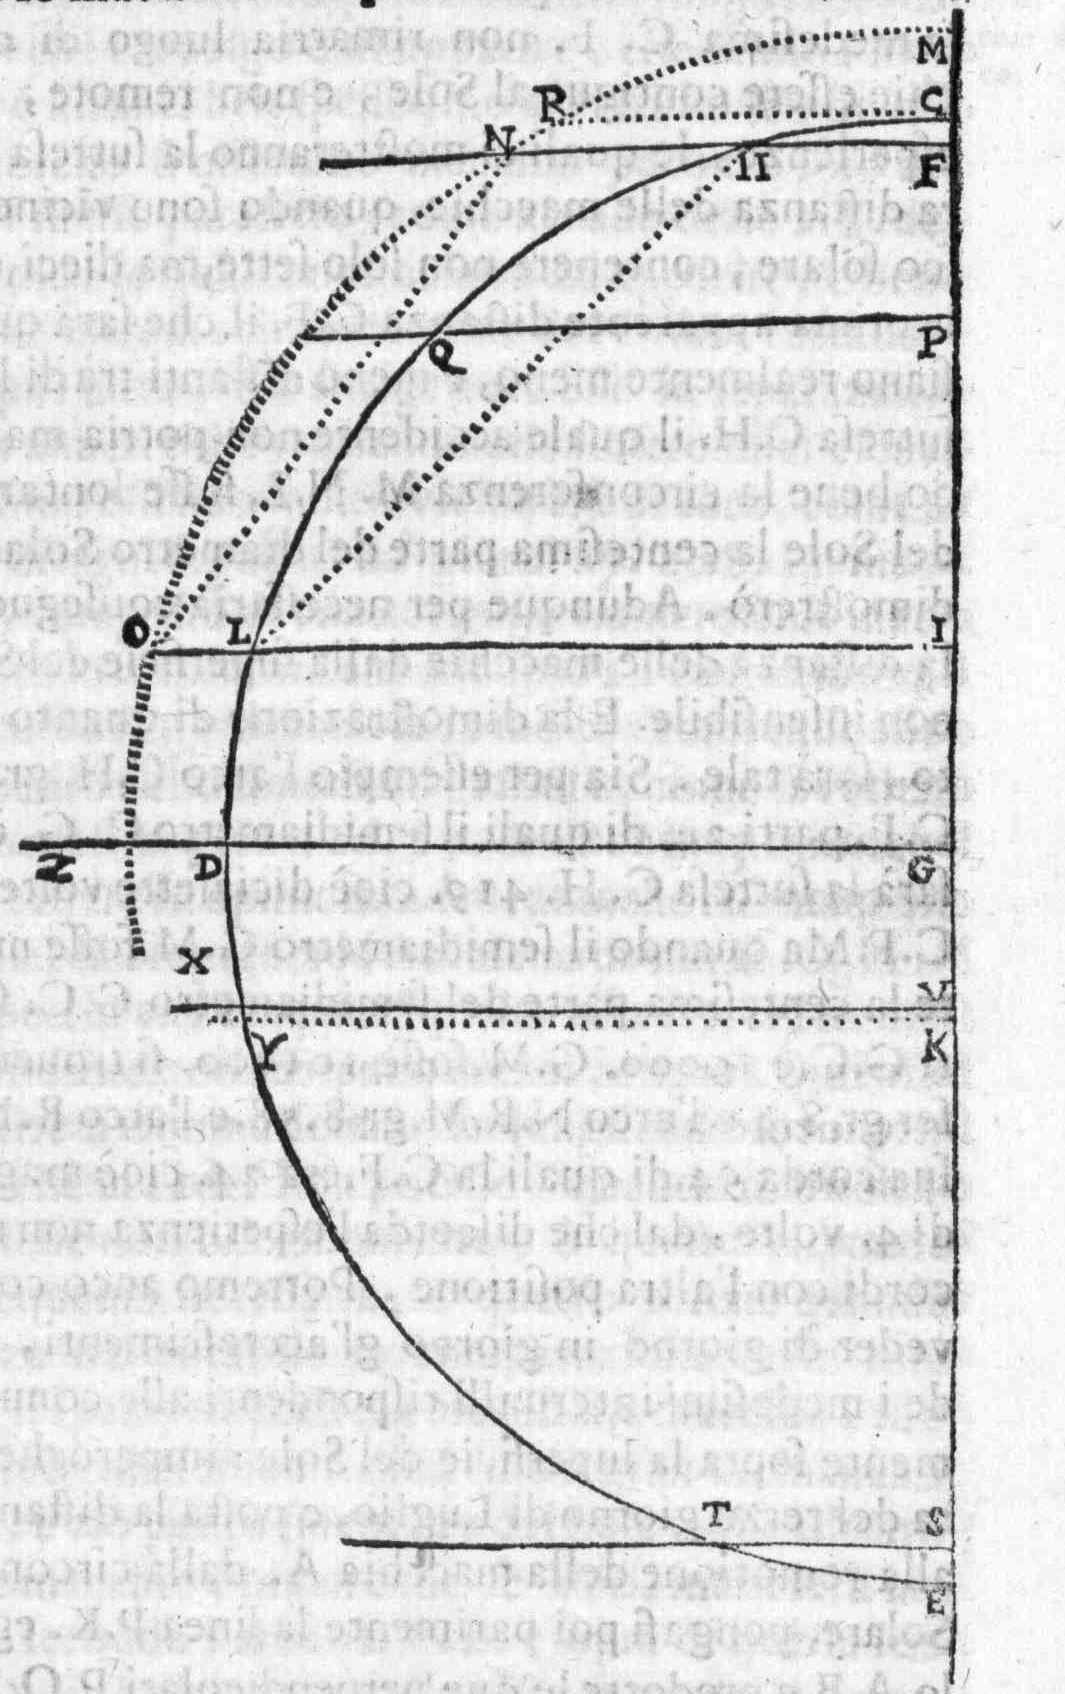
\includegraphics[width=0.8\textwidth]{ART_Sierotowicz/Sierotowicz_img1.jpg} 
	\caption{Galileo’s Practical Method -- the projection on the observational plane of the segment between two sunspots.}
\end{figure}

\begin{figure}[h]
	\centering
	\includegraphics[width=1\textwidth]{ART_Sierotowicz/Sierotowicz_img2.tif} 
	\caption{Galileo’s observation on the 1\textsuperscript{st} of July 1613.}
\end{figure}

\begin{figure}[h]
	\centering
	\includegraphics[width=1\textwidth]{ART_Sierotowicz/Sierotowicz_img3.tif} 
	\caption{Galileo’s observation on the 5\textsuperscript{th} of July 1613.}
\end{figure}

\begin{figure}[h]
	\centering
	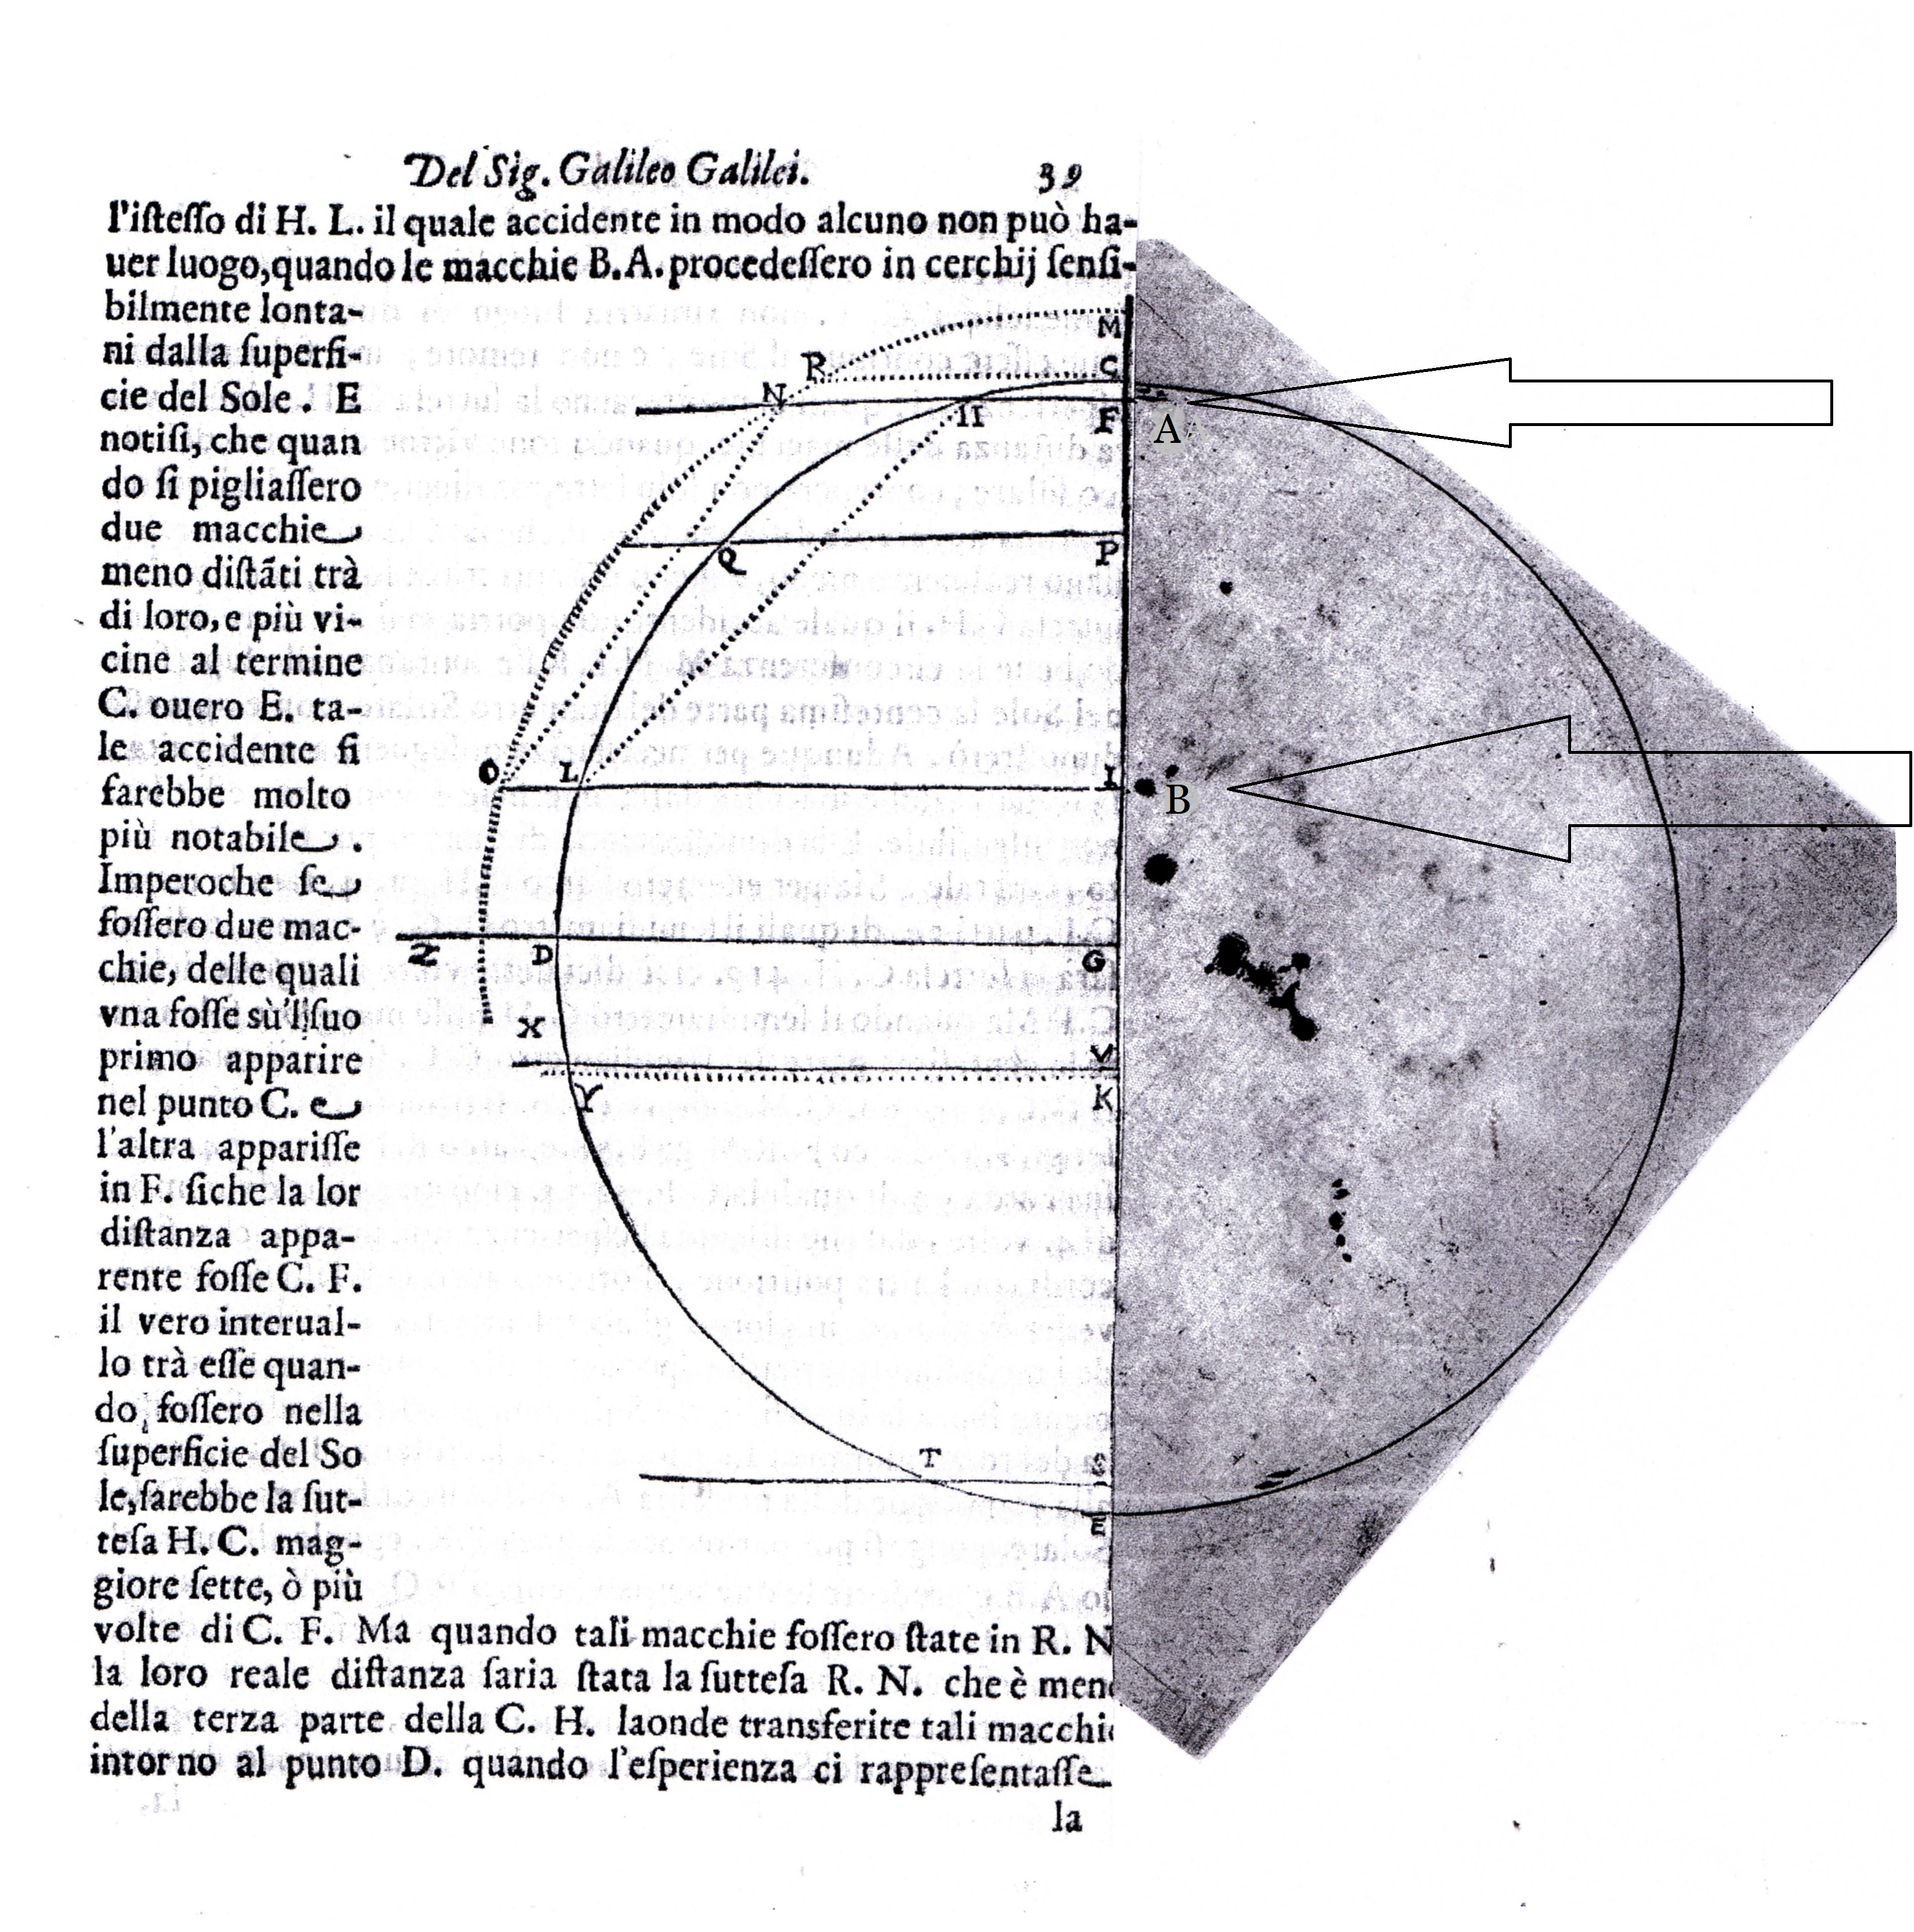
\includegraphics[width=1\textwidth]{ART_Sierotowicz/Sierotowicz_img4.jpg} 
	\caption{Sunspots observation, and its geometrical model for the 1\textsuperscript{st} of July 1613. The reconstruction
		by the Author.}
\end{figure}

\begin{figure}[h]
	\centering
	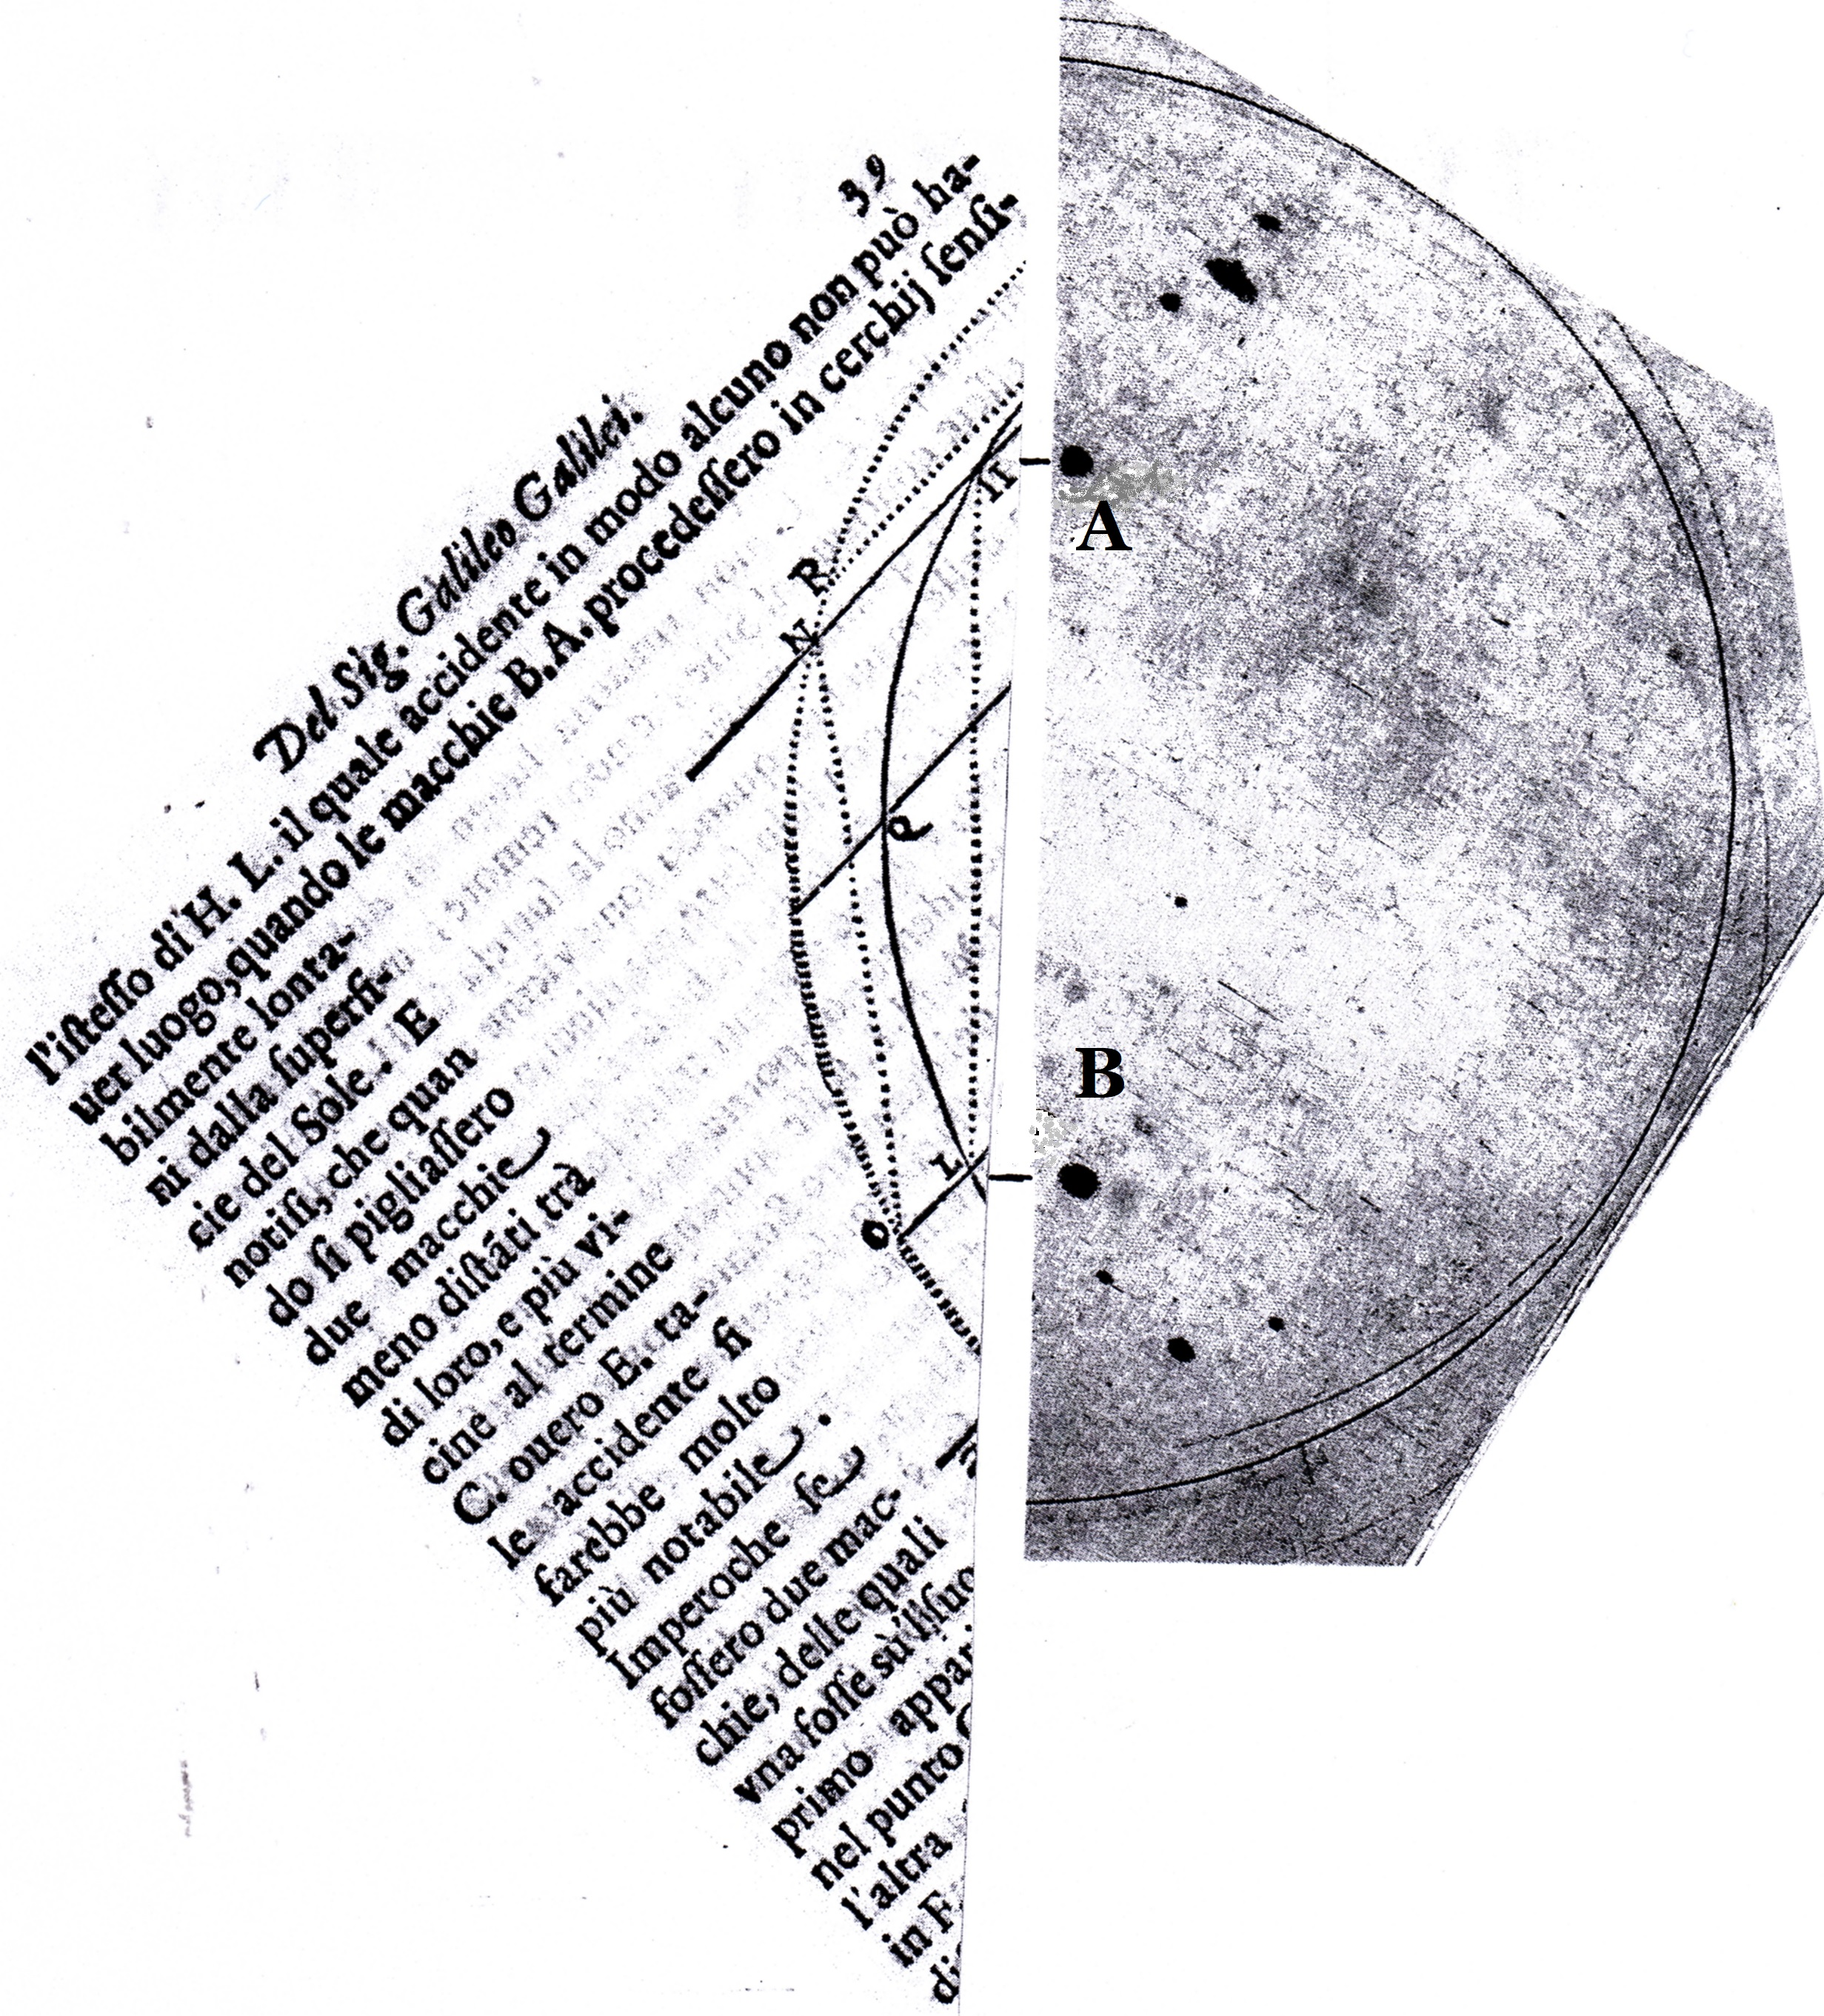
\includegraphics[width=1\textwidth]{ART_Sierotowicz/Sierotowicz_img5.jpg} 
	\caption{Sunspots observation, and its geometrical model for the 5\textsuperscript{th} July. The reconstruction by the
		Author.}
\end{figure}



\begin{bibliography}


\bibitem{camerota_galileo_2004}

\bibitem{camilleri_knowing_2015}

\bibitem{craik_nature_1943}

\bibitem{fantoli_galileo:_2003}

\bibitem{galilei_sunspots_2010}

\bibitem{heilbron_galileo_2010}

\bibitem{nersessian_theoreticians_1992}

\bibitem{nersessian_creating_2008}

\bibitem{palmerino_discussing_2018}

\bibitem{palmieri_mental_2003}

\bibitem{galilei_sunspots_2010-1}

\bibitem{shea_galileo_1970}

\bibitem{sierotowicz_o_2013}

\bibitem{stuart_routledge_2018}

\bibitem{succi_big_2019}

\bibitem{galilei_istoria_1613}

\bibitem{favaro_opere_1895}


\end{bibliography}



\end{artengenv}